% This work is made available under the terms of the
% Creative Commons Attribution-ShareAlike 4.0 license,
% http://creativecommons.org/licenses/by-sa/4.0/.
%
% Version: $Revision$

\documentclass[a4paper]{book}

\usepackage{wrapfig}
\usepackage{graphicx}
\usepackage{hyperref}
\usepackage{multirow}
\usepackage{scalefnt}
\usepackage{tikz}

% watermark -- for draft stage
\usepackage[firstpage]{draftwatermark}
\SetWatermarkLightness{0.9}
\SetWatermarkScale{5}

% Copyright (c) 2009 by the University of Waikato, Hamilton, NZ. 
% This work is made available under the terms of the 
% Creative Commons Attribution-ShareAlike 4.0 license,
% http://creativecommons.org/licenses/by-sa/4.0/.
%
% Version: $Revision: 5479 $

\newenvironment{tight_itemize}{
\begin{itemize}
  \setlength{\itemsep}{1pt}
  \setlength{\parskip}{0pt}
  \setlength{\parsep}{0pt}}{\end{itemize}
}

\newenvironment{tight_enumerate}{
\begin{enumerate}
  \setlength{\itemsep}{1pt}
  \setlength{\parskip}{0pt}
  \setlength{\parsep}{0pt}}{\end{enumerate}
}

% if you just need a simple heading
% Usage:
%   \heading{the text of the heading}
\newcommand{\heading}[1]{
  \vspace{0.3cm} \noindent \textbf{#1} \newline
}

\newcommand{\icon}[1]{\tikz[baseline=-3pt]\node[inner sep=0pt,outer sep=0pt]{\includegraphics[height=1.1em]{#1}};}


\title{
  \textbf{ADAMS} \\
  {\Large \textbf{A}dvanced \textbf{D}ata mining \textbf{A}nd \textbf{M}achine
  learning \textbf{S}ystem} \\
  {\Large Module: adams-webservice} \\
  \vspace{1cm}
  
\includegraphics[width=2cm]{images/webservice-module.png} \\
}
\author{
  Peter Reutemann
}

\setcounter{secnumdepth}{3}
\setcounter{tocdepth}{3}

\begin{document}

\begin{titlepage}
\maketitle

\thispagestyle{empty}
\center
\begin{table}[b]
	\begin{tabular}{c l l}
		\parbox[c][2cm]{2cm}{\copyright 2012-2017} &
		\parbox[c][2cm]{5cm}{
\includegraphics[width=5cm]{images/coat_of_arms.pdf}} \\
	\end{tabular}
	
\includegraphics[width=12cm]{images/cc.png} \\
\end{table}

\end{titlepage}

\tableofcontents
\listoffigures
%\listoftables

% %%%%%%%%%%%%%%%%%%%%%%%%%%%%%%%%%%
\chapter{Introduction}
The power of web-services \cite{webservice} lies in the fact that it decouples
software frameworks and it is possible to communicate without having to worry
about implementation or technology that each of the frameworks uses (see 
Figure \ref{webservices}). 

The \textit{adams-webservice} provides SOAP \cite{soap} web-service support using the Apache CXF
framework \cite{cxf}. ADAMS uses the approach to generate code on-the-fly based on a 
WSDL file \cite{wsdl}. This is also called \textit{WSDL first}.

If you already have existing code, then you can use Apache CXF as well to 
generate the WSDL from your code. See \cite{cxf-contract-first} on how to do
this.

\begin{figure}[htb]
  \centering
  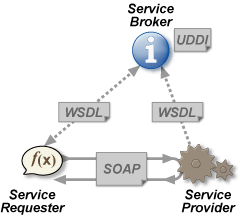
\includegraphics[width=6.0cm]{images/webservices.png}
  \caption{Webservice schema.}
  \label{webservices}
\end{figure}

%%%%%%%%%%%%%%%%%%%%%%%%%%%%%%%%%%%
\chapter{Creating a web-service}
Creating a web-service involves the following steps:
\begin{tight_enumerate}
	\item Define the WSDL for the web-service.
	\item Create a new ADAMS module, add the \textit{adams-webservice} artifacts
	as dependencies.
	\item Place your WSDL in the \texttt{src/main/resources/wsdl} directory
	(best to create a sub-directory there, e.g., \texttt{mywsdl}).
	\item Configure the code-generation using the WSDL as basis.
	\item Implementing the web-service functionaliy that processes the 
	data (server and client).
\end{tight_enumerate}

\section{Defining the WSDL}
If you start from scratch with a WSDL definition, check out the tutorial
at \cite{wsdl-tutorial}. On the other hand, if you already have existing
code, then refer to \cite{cxf-contract-first} on how to generate a WSDL from 
your code.

\section{Creating a new module}
For more details on this, please refer to the manual of the \textit{adams-core}
module. In the \textit{Developing with ADAMS} part, see section 
\textit{Creating a new module}.

\section{Configuring code-generation}
Now you need to configure your \textit{pom.xml} file to generate code from
the WSDL on-the-fly. You need to configure the \textit{cxf-codegen-plugin}
build plugin, i.e., where the WSDL is located and what code to generate
(you might have a bindings XML file as well).

The following \texttt{pom.xml} snippet shows how to do this for the Apache
CXF \textit{customer service} example (see ``wsdl\_first'' example in the 
CXF download). The WSDL \texttt{CustomerService.wsdl} is located in 
\texttt{src/main/resources/wsdl/customerservice} and also comes with a 
bindings file \texttt{CustomerService-binding.xml} in the same directory.
We want to to create \textit{JAX-WS 2.1} compatible code out of it, which we
define using the \textit{-frontend} parameter. And since we want to create
Java code from the WSDL, we need to use goal \textit{wsdl2java}.
{\scriptsize
\begin{verbatim}
  <plugin>
    <groupId>org.apache.cxf</groupId>
    <artifactId>cxf-codegen-plugin</artifactId>
    <executions>
      <execution>
        <id>generate-sources</id>
        <phase>generate-sources</phase>
        <configuration>
          <wsdlOptions>
            <wsdlOption>
              <wsdl>src/main/resources/wsdl/customerservice/CustomerService.wsdl</wsdl>
              <wsdlLocation>classpath:wsdl/customerservice/CustomerService.wsdl</wsdlLocation>
              <bindingFiles>
                <bindingFile>src/main/resources/wsdl/customerservice/CustomerService-binding.xml</bindingFile>
              </bindingFiles>
              <frontEnd>jaxws21</frontEnd>
            </wsdlOption>
          </wsdlOptions>
        </configuration>
        <goals>
          <goal>wsdl2java</goal>
        </goals>
      </execution>
    </executions>
  </plugin>
\end{verbatim}
}

\section{Implementing the web-service}
Depending on your web-service you might have to implement the following
functionality:
\begin{tight_itemize}
	\item {Server} -- processes requests and sends back responses
	\item {Client} -- queries a server and processes the response
\end{tight_itemize}
The following sections explain each in detail.

\subsection{Dummy}
In order to get a dummy implementation generated, you can use the 
\texttt{wsdl2java} tool that comes with the \textit{Apache CXF} binary 
distribution. The dummy implementation is generated using the \texttt{-impl} 
parameter. Here is an example of generating JAX-WS 2.1 compatible output
for the customer service example WSDL:
{\scriptsize
\begin{verbatim}
./apache-cxf-2.6.3/bin/wsdl2java 
    -impl
    -server
    -client
    -fe jaxws21 
    -wsdlLocation "classpath:wsdl/customerservice/CustomerService.wsdl" 
    CustomerService.wsdl
\end{verbatim}}
The \texttt{-wsdlLocation} parameter indicates where the Apache CXF code
will find the WSDL at runtime. This gets added to the \texttt{wsdlLocation}
attribute of the \texttt{javax.jws.WebService} annotation.

Three generated files are basically of interest here:
\begin{tight_itemize}
	\item \textit{CustomerService\_CustomerServicePort\_Client.java} -- client
	code for that shows how to query the webservice.
	\item \textit{CustomerService\_CustomerServicePort\_Server.java} -- server
	code for starting the web-service, makes use of \textit{CustomerServiceImpl.java}.
	\item \textit{CustomerServiceImpl.java} -- the dummy implementation that
	processes the incoming request from the client and generates a response.
\end{tight_itemize}
Parts of this example code will be used in implementing plugins for ADAMS.

\subsection{Server}
Your server component needs to implement the following interface:
\begin{verbatim}
adams.flow.webservice.WebServiceProvider
\end{verbatim}
It is easiest to implement your class in the same package, otherwise you need
to tell ADAMS where to find your classes (see section \textit{Dynamic class 
discovery} in the \textit{adams-core} manual).

For convenience, you can simply sub-class the following abstract superclass:
\begin{verbatim}
adams.flow.webservice.AbstractWebServiceProvider
\end{verbatim}
If you need to process the query data with a sub-flow, see section 
\ref{webservice_callable_transformer}.

Using the example code generated earlier, we can now implement out server
component. You only need to specify the default URL that the web-service
gets published under (\texttt{getDefaultURL()}), how to start the web-service
(\texttt{doStart()}) and how to stop it again (\texttt{doStop()}).

Here is a basic implementation\footnote{com.example.customerservice.flow.CustomerServiceWS,
adams-webservice-server.flow}:
{\scriptsize
\begin{verbatim}
public class CustomerServiceWS extends AbstractWebServiceProvider {

  protected EndpointImpl m_Endpoint;
  
  @Override
  public String globalInfo() {
    return "Provides a customer service webservice.";
  }

  @Override
  public String getDefaultURL() {
    return "http://localhost:9090/CustomerServicePort";
  }

  @Override
  protected void doStart() throws Exception {
    m_Endpoint  = (EndpointImpl) Endpoint.publish(getURL(), new CustomerServiceImpl(this));
  }

  @Override
  protected void doStop() throws Exception {
    if (m_Endpoint != null) {
      m_Endpoint.getServer().stop();
      m_Endpoint = null;
    }
  }
}
\end{verbatim}}

As you can see, we make use of the dummy implementation created by Apache CXF
in the \texttt{doStart()} method:
\begin{verbatim}
  new CustomerServiceImpl(this)
\end{verbatim}

By default, the ``dummy implementation'' class (\textit{CustomerServiceImpl})
only has a default constructor. In order to give it access to the webservice
and integrate it with ADAMS, we need to add a custom constructor, to link it to the
webservice that it uses:
\begin{verbatim}
    /** the ADAMS owner. */
    protected CustomerServiceWS m_Owner;

    /** Initializes the service. */
    public CustomerServiceImpl(CustomerServiceWS owner) {
      super();
      m_Owner = owner;
    }
\end{verbatim}

\subsection{Client}
For the client component, you need to implement this interface:
\begin{verbatim}
adams.flow.webservice.WebServiceClient
\end{verbatim}
Depending on whether your client can take input or generates output, you need
to implement the following interfaces as well:
\begin{tight_itemize}
	\item \textit{WebServiceClientConsumer} -- accepts input, which will get
	forwarded to the web-service.
	\item \textit{WebServiceClientProducer} -- generates output based on the
	webs-service response.
\end{tight_itemize}
In order to make development of new web-service components faster, a bunch
of abstract classes is already available:
\begin{tight_itemize}
	\item \textit{AbstractWebServiceClientSource} -- for a client that outputs
	the web-service reponse\footnote{adams-webservice-client\_as\_source.flow}.
	\item \textit{AbstractWebServiceClientTransformer} -- the client queries the 
	web-service with data it receives and outputs the web-service 
	reponse\footnote{adams-webservice-client\_as\_transformer.flow}.
	\item \textit{AbstractWebServiceClientSink} -- sends the incoming data
	to the web-service and generates no output\footnote{adams-webservice-client\_as\_sink.flow}.
\end{tight_itemize}
If some of the data requires pre- or post-processing with a sub-flow, check
out section \ref{webservice_callable_transformer} for more details on how to do
this.

Using the previous customer service example again, we can now generate a
transformer client that queries the web-service with a customer name and
then outputs the results. You need to implement the following methods:
\begin{tight_itemize}
	\item \texttt{getWsdlLocation()} -- where to find the WSDL.
	\item \texttt{setRequestData(T)} -- for setting the query data.
	\item \texttt{doQuery()} -- how to perform the query.
	\item \texttt{hasResponseData()} -- whether there is any response data
	available.
	\item \texttt{getResponseData()} -- for obtaining the response data.
	\item \texttt{accepts()} -- what type of input data the client accepts.
	\item \texttt{generates()} -- what type of output data the client generates.
\end{tight_itemize}

Here is an example 
implementation\footnote{com.example.customerservice.flow.CustomersByName}:
{\scriptsize
\begin{verbatim}
public class CustomersByName extends AbstractWebServiceClientTransformer<String,String> {
  
  protected String m_CustomerName;  // the name of the customers to look up
  protected String m_ProvidedCustomerName;  // the customer name received by actor
  protected List<Customer> m_Customers;  // the list of customers that were obtained from webservice

  @Override
  public String globalInfo() {
    return "Returns customer names.";
  }

  @Override
  public Class[] accepts() {
    return new Class[]{String.class};
  }

  @Override
  public void setRequestData(String value) {
    m_ProvidedCustomerName = value;
  }

  @Override
  protected URL getWsdlLocation() {
    return getClass().getClassLoader().getResource("wsdl/customerservice/CustomerService.wsdl");
  }

  @Override
  protected void doQuery() throws Exception {
    m_Customers = null;
    CustomerServiceService customerServiceService = new CustomerServiceService(getWsdlLocation());
    CustomerService customerService = customerServiceService.getCustomerServicePort();
    WebserviceUtils.configureClient(
	m_Owner,
	customerService,
	m_ConnectionTimeout,
	m_ReceiveTimeout,
	(getUseAlternativeURL() ? getAlternativeURL() : null),
	m_InInterceptor,
	m_OutInterceptor);
    WebserviceUtils.enableSchemaValidation(((BindingProvider) customerService));
    m_Customers = customerService.getCustomersByName(m_ProvidedCustomerName);
    m_ProvidedCustomerName = null;
  }

  @Override
  public Class[] generates() {
    return new Class[]{String.class};
  }
  
  public boolean hasResponseData() {
    return (m_Customers != null) && (m_Customers.size() > 0);
  }

  @Override
  public String getResponseData() {
    String result = m_Customers.get(0).getCustomerId() + ": " + m_Customers.get(0).getName() 
        + ", " + Utils.flatten(m_Customers.get(0).getAddress(), " ");
    m_Customers.remove(0);
    return result;
  }
}
\end{verbatim}
}

\subsection{Callable transformer support}
\label{webservice_callable_transformer}
In order to utilize the power of the workflow, you can also process data,
in the server and client alike, using a callable transformer.
If your component needs to take advantage of such functionality, it needs to
implement the \texttt{CallableTransformerSupport} interface. For convenience,
there are already abstract classes in place:
\begin{tight_itemize}
	\item \textit{AbstractWebServiceProviderWithCallableTransformer} -- if the server needs
	to process the incoming data with a sub-flow.
	\item \textit{AbstractWebServiceClientSourceWithCallableTransformer} -- a 
	source client that pre-processes the query or post-processes the response.
	\item \textit{AbstractWebServiceClientTransformerWithCallableTransformer} --
	a transformer client that post-processes the 
	response\footnote{adams-webservice-client\_as\_transformer-callable\_transformer.flow}.
	\item \textit{AbstractWebServiceClientSinkWithCallableTransformer} -- a
	sink client that pre-processes the incoming data before querying the service.
\end{tight_itemize}
You can use the \texttt{applyTransformer} method to transform the data.

%%%%%%%%%%%%%%%%%%%%%%%%%%%%%%%%%%%
\chapter{Flow}
This module contains generic actors in which you can simply plug your 
web-services that you have implemented. In the following a short overview.

The following standalones are available:
\begin{tight_itemize}
	\item \textit{WSServer} -- runs a web-service. waiting for 
	requests\footnote{adams-webservice-server.flow}.
\end{tight_itemize}
The following sources are available:
\begin{tight_itemize}
	\item \textit{WSSource} -- queries a web-service and forwards the received 
	data\footnote{adams-webservice-client\_as\_source.flow}.
\end{tight_itemize}
The following transformers are available:
\begin{tight_itemize}
	\item \textit{WSTransformer} -- sends the data it receives to a web-service
	and forwards the data from the response in 
	turn\footnote{adams-webservice-client\_as\_transformer.flow}\footnote{adams-webservice-client\_as\_transformer-callable\_transformer.flow}.
\end{tight_itemize}
The following sinks are available:
\begin{tight_itemize}
	\item \textit{WSSink} -- simply sends data to a web-service\footnote{adams-webservice-client\_as\_sink.flow}.
\end{tight_itemize}

%%%%%%%%%%%%%%%%%%%%%%%%%%%%%%%%%%%
\chapter{Messages}
The following sections explain how SOAP messages can be intercepted (in- and
outgoing ones) and also replayed. This is especially useful when debugging
webservices.

\section{Interception}
Webservice clients and servers can take advantage of the same interceptors.

\noindent The following generators for \textit{incoming} interceptors are available:
\begin{tight_itemize}
  \item \textit{BaseLoggingGenerator} -- simply outputs the message using the
  ADAMS logging framework.
  \item \textit{EnqueueGenerator} -- forwards the messages to the specified
  queue for further processing.
  \item \textit{LogFileGenerator} -- appends the messages to the specified log file.
  \item \textit{NullGenerator} -- does nothing (default).
  \item \textit{XMLLoggingGenerator} -- outputs the message as XML, either via
  logging or to a file.
\end{tight_itemize}

\noindent The following generators for \textit{outgoing} interceptors are available:
\begin{tight_itemize}
  \item \textit{BaseLoggingGenerator} -- simply outputs the message using the
  ADAMS logging framework.
  \item \textit{EnqueueGenerator} -- forwards the messages to the specified
  queue for further processing.
  \item \textit{LogFileGenerator} -- appends the messages to the specified log file.
  \item \textit{NullGenerator} -- does nothing (default).
  \item \textit{XMLLoggingGenerator} -- outputs the message as XML, either via
  logging or to a file.
\end{tight_itemize}


\section{Simulation}
Messages collected using one of the \textit{XMLLoggingGenerator} instances or
hand-coded ones can be replayed again rather easily. This is great for
debugging the handling of requests, without relying on an actual sender
transmitting the requests.

For sending, you can use one of the following approaches:
\begin{tight_itemize}
  \item \textit{SoapUI}\cite{soapui} -- an application for testing SOAP and REST
  \item Workflow using the \textit{HttpRequest} transformer\footnote{adams-webservice-simulate.flow}
\end{tight_itemize}

\noindent For the second approach to work, not only the URL of the webservices
has to be supplied, but also additional HTTP headers (the payload itself is the
content of the XML file). The following headers should be included:
\begin{tight_itemize}
  \item \texttt{Content-Type=text/xml}
  \item \texttt{Content-Length=length}
  \item \texttt{SOAPAction=XYZ}
\end{tight_itemize}
The \textit{SOAPAction} header is specific to the webservice. Some webservices
might not require it at all and therefore can be left empty. This action is
output in the default logging information in the console, just search for the
\textit{SOAPAction:} text in the output.


%%%%%%%%%%%%%%%%%%%%%%%%%%%%%%%%%%%
% Copyright (c) 2009-2012 by the University of Waikato, Hamilton, NZ. 
% This work is made available under the terms of the 
% Creative Commons Attribution-ShareAlike 4.0 license,
% http://creativecommons.org/licenses/by-sa/4.0/.
%
% Version: $Revision$

\begin{thebibliography}{999}
	% to make the bibliography appear in the TOC
	\addcontentsline{toc}{chapter}{Bibliography}

    % references
	\bibitem{adams}
		\textit{ADAMS} -- Advanced Data mining and Machine learning System \\
		\url{https://adams.cms.waikato.ac.nz/}{}
		
	\bibitem{heatmap}
		\textit{Heat map} -- WikiPedia article \\
		\url{http://en.wikipedia.org/wiki/Heat_map}{}

\end{thebibliography}


\end{document}
